%%%%%%%%%%%%%%%%%%%%%%%%%%%%%%%%%%%%%%%%%%%%%%%%%%%%%%%%%%%%%%%%%%%%%%%%%%%%%%%%%%%%%%%%%%%%%%%%%%%%%%%%%%%%%%%%%%%%%%%%%%%%%%%%%%%%%%%%
% This is just a template to use when submitting manuscripts to Frontiers, it is not mandatory to use frontiers.cls nor frontiers.tex  %
%%%%%%%%%%%%%%%%%%%%%%%%%%%%%%%%%%%%%%%%%%%%%%%%%%%%%%%%%%%%%%%%%%%%%%%%%%%%%%%%%%%%%%%%%%%%%%%%%%%%%%%%%%%%%%%%%%%%%%%%%%%%%%%%%%%%%%%%

\documentclass{frontiersENG} % for Engineering articles
%\documentclass{frontiersSCNS} % for Science articles
%\documentclass{frontiersMED} % for Medicine articles

\usepackage{url,lineno}
\linenumbers

\usepackage{graphicx}

% Leave a blank line between paragraphs in stead of using \\

\copyrightyear{}
\pubyear{}

\def\journal{Neuroinformatics}%%% write here for which journal %%%
\def\DOI{}
\def\articleType{Research Article}
\def\keyFont{\fontsize{8}{11}\helveticabold }
\def\firstAuthorLast{Sample {et~al.}} %use et al only if is more than 1 author
\def\Authors{Matthew McCormick\,$^{1,*}$,
  Xiaxiao Liu\,$^{1}$,
  Julien Jomier\,$^{2}$,
  Charles Marion\,$^{2}$,
  Joshua Carp\,$^{3}$,
  and Luis Ibanez\,$^1$}
% Affiliations should be keyed to the author's name with superscript numbers and be listed as follows: Laboratory, Institute, Department, Organization, City, State abbreviation (USA, Canada, Australia), and Country (without detailed address information such as city zip codes or street names).
% If one of the authors has a change of address, list the new address below the correspondence details using a superscript symbol and use the same symbol to indicate the author in the author list.
\def\Address{$^{1}$Medical Computing Group, Kitware Inc, Clifton Park, NY, USA\\
$^{2}$Medical Computing Group, Kitware Inc, Lyon, France\\
$^{3}$University of Michigan, Ann Arbor, MI, USA\\
}
% The Corresponding Author should be marked with an asterisk
% Provide the exact contact address (this time including street name and city zip code) and email of the corresponding author
\def\corrAuthor{Luis Ibanez}
\def\corrAddress{Medical Computing Group, Kitware Inc, Clifton Park, NY, USA}
\def\corrEmail{luis.ibanez@kitware.com}

% \color{FrontiersColor} Is the color used in the Journal name, in the title, and the names of the sections


\begin{document}
\onecolumn
\firstpage{1}

\title[ITK Reproducible Research]{ITK Enabling Reproducible Research and Open Science}
\author[\firstAuthorLast ]{\Authors}
\address{}
\correspondance{}
\extraAuth{}% If there are more than 1 additional author, comment this line and uncomment the next one
%\extraAuth{corresponding Author2 \\ Laboratory X2, Institute X2, Department X2, Organization X2, Street X2, City X2 , State XX2 (only USA, Canada and Australia), Zip Code2, X2 Country X2, email2@uni2.edu}
\topic{Research Topic}

\maketitle
\begin{abstract}

\section{}
%As a primary goal, the abstract should render the general significance and conceptual advance of the work clearly accessible to a broad readership. References should not be cited in the abstract.
See the Summary Table at \\ \url{http://www.frontiersin.org/}\texttt{\journal}\url{/authorguidelines} \\for abstract requirement and length according to article type.


\tiny
 \keyFont{ \section{Keywords:} Reproducibilty ITK InsightToolkit Review Text Text Text Text } %All article types: you may provide up to 8 keywords; at least 5 are mandatory.
\end{abstract}


\section{Introduction}

% For Original Research Articles, Clinical Trial Articles, and Technology Reports the introduction should be succinct, with no subheadings.
%
%For Clinical Case Studies the Introduction should include symptoms at presentation, physical exams and lab results.
%

The essential feature of the scientific method is the practice of verification
of reproducibility.

This verification is better performed by independent parties, and to be
trustable, it must be performed multiple times. These are the essential
principles that guided the establishment of the early scientific societies in
the 17th century, such as the Royal Society and the Lincean Academy.

The Motto of the Royal Society:  "Nullius in Verba" roughly translates as "Take
nobody's word for it", and "...it is an expression of the determination of
Fellows to withstand the domination of authority and to verify all statements
by an appeal to facts determined by experiment". It was this approach to
scientific research what triggered the enlightenment of the 17th century.

Unfortunately today, the economics of how we fund modern science had led
research organizations to discard the true practice of the scientific method
and instead engage in practices that are closer to the marketing and branding
of manufactured products. Instead of attention to the practice of
reproducibility verification, Journals and Conferences have obsessed with
Novelty. Journals and Conferences have confused their mission of dissemination
of scientific information with an attempt to play the role of a surrogate of
the patent office.

In the process, Journals and Conferences have confused the profession of
scientific researcher with the profession of inventor. These are indeed two
very different vocations, although it is common to find them intermixed when
researchers express traits of invention in the process of crafting the methods
and tools that are needed to further their scientific quest. for example
Antonie Leeuwenhoek behave as a scientist when making the first observation of
micro-organisms in 1665, and behave as an inventor when crafting the unique
microscopes that he used for his observations. The duality of these two
profession is quite clearly illustrated in this case by the fact that
Leeuwenhoek generously share the findings of his observations of
microorganisms, but kept secret the technical details of the construction of
his microscopes. As a consequence, his scientific work gave birth to the field
of microbiology, while his microscope building techniques were taken with him
to his grave, and it took 150 years for microscopes of similar quality to be
re-developed.

The large majority of research activity today is focused on generating novelty,
and only in exceptional cases, concerned with the verification of
reproducibility. The practice of peer-review has been assumed to be a suitable
replacement for the verification of reproducibility. A mistake by which
experimental work has been replaced by thought experiments and opinion-based
evaluations that do little to further the scientific enterprise. This drift has
denigrated, what used to be scientific work, back into the practice of the
"natural philosophy" in which we simply imagine models of the natural word and
evaluate them based on aesthetic appeals and desire of self-consistency.

The Insight Toolkit (ITK) has made possible to restore the true practice of the
scientific method in the field of medical image analysis. By providing a common
platform in which image analysis algorithms and processing techniques can be
implemented and can be freely disseminated. ITK empowers all to verify the
experimental work of image analysis research activities. This of course, to
requires that researchers adhere to the true practice of the scientific method
and publish the full details of their methodology, including the source code,
data, parameters and auxiliary documents that are required for a third party to
independently repeat the work and verify the findings.

The ITK community created in 2005 a scientific journal, truly fulfilling the
practice of the scientific method, where all articles are required to provide
the full set of source code, data and parameters needed to reproduce the
finding of the authors. These materials are immediately made available to
readers and reviewers, empowering them to indeed perform such verification with
minimal effort and minimal losses of information.

Other Journals, in particular Frontiers, PLoS, and more recently Nature, have
embraced this restoration of the true practice of the scientific method.  With
the support of the Reproducible Research movement, these progressive
publication venues are creating the conditions for a new age of enlightenment
in which the methodologies of practical research work will not be subject to
secrecy, nor be subject to the veil of suspicion that many incidents of
scientific fraud, and data manufacturing that have left us with in recent
months.

The open source nature of ITK, the open access nature of the Insight Journal,
and the public sharing of open data that is enabled by the Midas Platform in
the ITK community, are the three pillars of Open Science that are transforming
the way scientific research is done today.

The technological challenges of reproducibility have all been solved. We now
require a cultural change by which we must make simply unacceptable that any
article in the domain of medical image analysis be published without the full
set of source code, data and parameters that will enable an independent group
to replicate the process and verify or refute the findings.




%\begin{methods}
\section{Material \& Methods}

Text Text Text Text Text Text  Text Text Text Text Text Text Text Text Text  Text Text Text Text Text Text Text Text Text Text  Text Text Text Text Text Text  Text Text.  \cite{Neuro2013} might want to know about  text text text text Text Text Text Text  Text Text Text Text Text Text  Text Text. \citep{Gene2012} might want to know about  text text text text
Text Text Text Text Text Text  Text Text Text Text Text Text Text Text Text  Text Text Text Text Text Text Text Text Text Text  Text Text Text Text Text Text  Text Text.  \cite{Neurobot2013} might want to know about  text text text text


\subsection{Original Research Articles, Clinical Trial Articles, and Technology Reports}

For Original Research Articles, Clinical Trial Articles, and Technology Reports the following sections are mandatory:

\begin{itemize}
%for bulleted list, use itemize
\item Introduction: Succinct, with no subheadings.
\item Materials and Methods: This section may be divided by subheadings. This section should contain sufficient detail so that when read in conjunction with cited references, all procedures can be repeated.
\item Results: This section may be divided by subheadings. Footnotes should not be used and have to be transferred into the main text.
\item Discussion: This section may be divided by subheadings. Discussions should cover the key findings of the study: discuss any prior art related to the subject so to place the novelty of the discovery in the appropriate context; discuss the potential short-comings and limitations on their interpretations; discuss their integration into the current understanding of the problem and how this advances the current views; speculate on the future direction of the research and freely postulate theories that could be tested in the future.
\end{itemize}

Please note that the Material and Methods section can be placed in any of the following ways: before Results, before Discussion or after Discussion.



\textbf{Figure 1.}{ Enter the caption for your figure here.  Repeat as  necessary for each of your figures.}\label{fig:01}% Don't add the figures in the LaTeX files, please upload them when submitting the article. Frontiers will add the figures at the end of the provisional pdf.


\subsection{Clinical Case Studies}

For Clinical Case Studies the following sections are mandatory:

\begin{itemize}
%for bulleted list, use itemize
\item Introduction: Include symptoms at presentation, physical exams and lab results.
\item Background: This section may be divided by subheadings. Include history and review of similar cases.
\item Results: This section may be divided by subheadings. Include diagnosis and treatment.
\item Concluding Remarks
\end{itemize}

Please note that the Material and Methods section can be placed in any of the following ways: before Results, before Discussion or after Discussion.

%\end{methods}



\section{Results}

Frontiers requires figures to be submitted individually, in the same order as they are referred to in the manuscript. Figures will then be automatically embedded at the bottom of the submitted manuscript. Kindly ensure that each table and figure is mentioned in the text and in numerical order. Permission must be obtained for use of copyrighted material from other sources (including the web). Please note that it is compulsory to follow figure instructions. Figures which are not according to the guidelines will cause substantial delay during the production process.

\begin{table}[!t]
\processtable{Resolution Requirements for the figures\label{Tab:01}}
{\begin{tabular}{lllll}\toprule
Image Type & Description & Format & Color Mode & Resolution\\\midrule
Line Art & An image composed of lines and text,  & TIFF, EPS, JPEG & RGB, Bitmap & 900 - 1200 dpi\\
           & which does not contain tonal or shaded areas.& & &\\
           Halftone & A continuous tone photograph, which contains no text. & TIFF, EPS, JPEG & RGB, Grayscale & 300 dpi\\
Combination & Image contains halftone + text or line art elements. & TIFF, EPS, JPEG & RGB,Grayscale & 600 - 900 dpi\\\botrule
\end{tabular}}{This is a footnote}
\end{table}

\begin{equation}
\sum x+ y =Z\label{eq:01}
\end{equation}

\textbf{Table\ref{Tab:01}} shows the resolution requirements for the figures. The figures must be legible:
\begin{enumerate}
\item The smallest visible text is no less than 8 points in height, when viewed at actual size.
\item Solid lines are not broken up.
\item Image areas are not pixelated or stair stepped.
\item Text is legible and of high quality.
\item Any lines in the graphic are no smaller than 2 points width.
\end{enumerate}

\textbf{Figure 2.}{Enter the caption for your figure here.  Repeat as  necessary for each of your figures.}\label{fig:02}

\subsection{Open Review System: Gerrit Review}

In the three years that the community has applied the Gerrit Code review
system, << d['src/gerrit_results.json'].from_json()['changes'] >> changes have
been submitted to the review server and
<< d['src/gerrit_results.json'].from_json()['reviews'] >> were performed.
As a matter of policy, all merged changes should have at least one review,
but the number of iterations on a change varies flexibly depending on the
requirements. This results in a roughly negative exponential distribution in
revisions, as evident in the histogram of revisions in
Figure~\ref{fig:gerrit_patch_set_histogram}.  The highest number of reviews
for a single change was
<< d['src/gerrit_results.json'].from_json()['max_reviews'] >>.

Two direct but notable conclusions follow from this data. First, at least one
other person examined and reproduced a proposed code.  This certainly exceeds
publication systems where the code is never dissemminated, and it likely
exceeds validation systems where the code is published, but there is no
incentive or check that reviewers looked at it or applied it.
 
\begin{figure}
  \centering
    \includegraphics[width=0.5\textwidth]{gerrit_patch_set_histogram.eps}
    \caption{Histogram of the number of revisions (Patch Sets) for a given change.}
    \label{fig:gerrit_patch_set_histogram}
\end{figure}

\begin{figure}
  \centering
    \includegraphics[width=0.5\textwidth]{gerrit_fix_ups.eps}
    \caption{Fix-up commit percentage before and after peer code review.}
    \label{fig:gerrit_fix_ups}
\end{figure}

\begin{figure}
  \centering
    \showthe\textwidth
    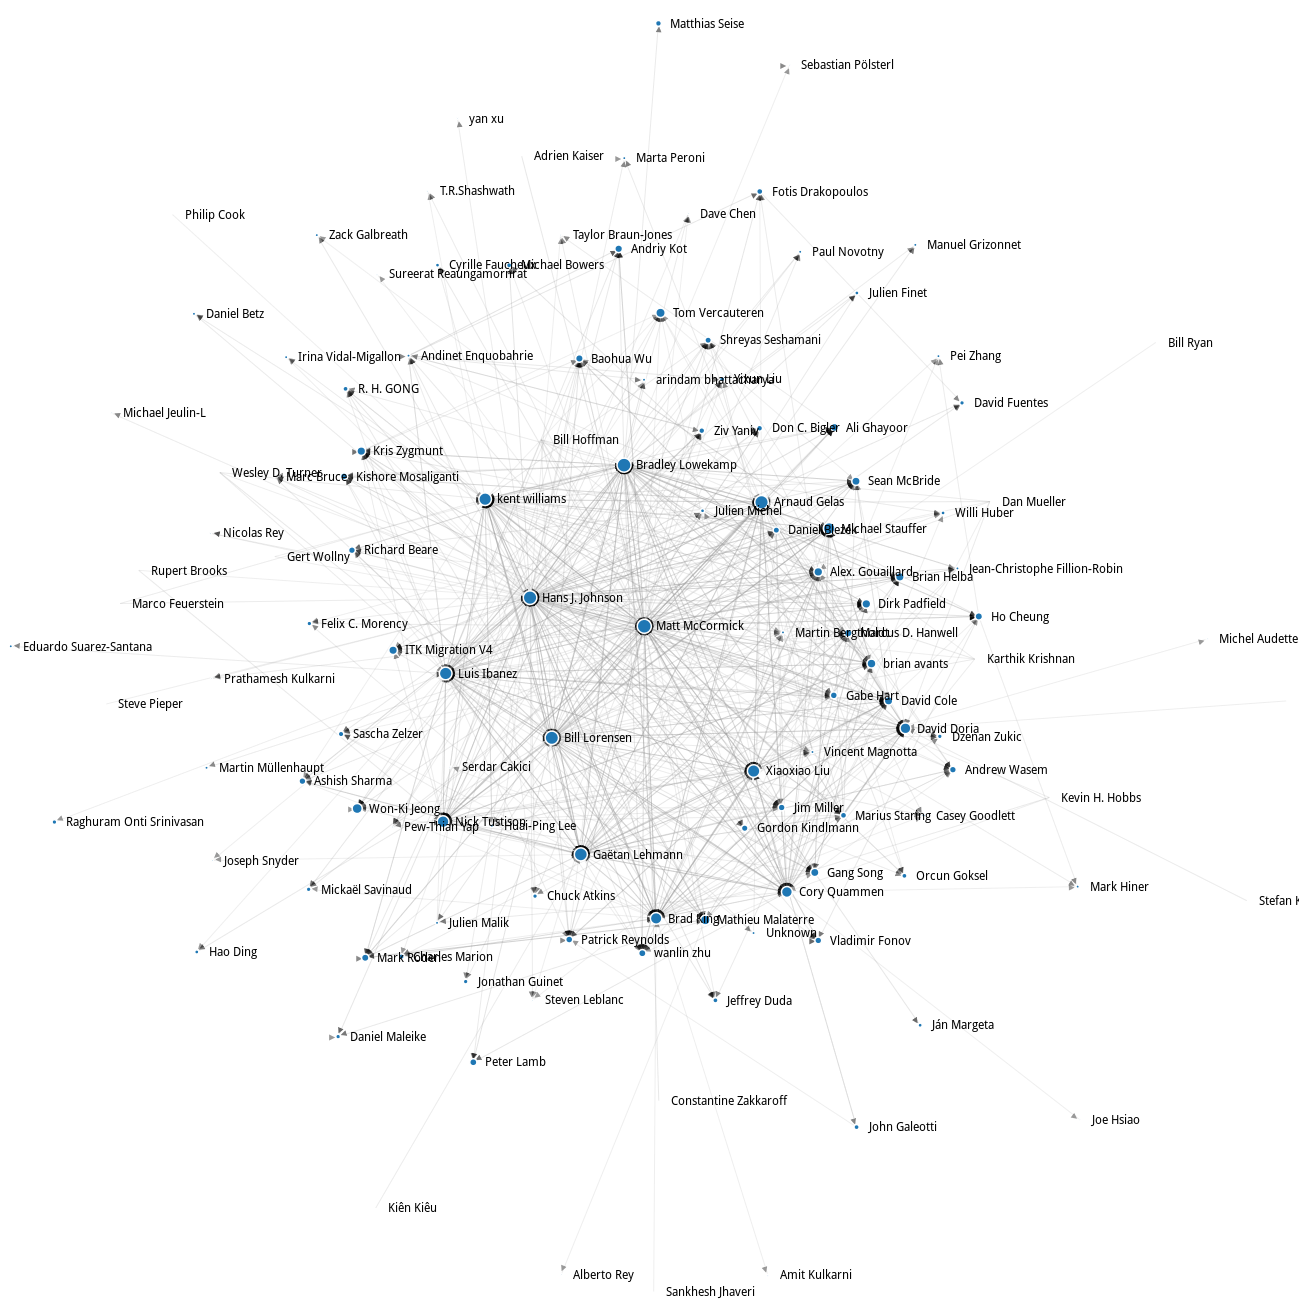
\includegraphics[width=1.0\textwidth]{GerritGraphRender.png}
    \caption{Peer code reviews.  Nodes are individual community members and
      size of the circle at the node is related to logarithm of the number of changes
      created by that community member.  The widths of the edges in this directed
      graph are proportional to the number of reviews performed.}
    \label{fig:gerrit_fix_ups}
\end{figure}

\section{Discussion}

Text Text Text Text Text Text  Text Text Text Text Text Text Text Text Text  Text Text Text Text Text Text Text Text Text Text.
Additional Requirements:
\subsection{Corrections}

Minor corrections to published articles can be communicated to the Frontiers Production Office at production.office@frontiersin.org. If you need to communicate important changes to an article please submit a General Commentary. Submit the article with the title "Erratum: Original Title of Article".

\subsection{Commentaries on Articles}

At the beginning of your manuscript provide the citation of the article commented on.

\subsection{Focused Reviews}

For Tier 2 invited Focused Reviews the sections Introduction, Material and Methods, Results, and Discussion are recommended. In addition the authors must submit a short biography of the corresponding author(s). This short biography has a maximum of 600 characters, including spaces.

A picture (5 x 5 cm, in *.tif or *.jpg, min 300 dpi) must be submitted along with the biography in the manuscript and separately during figure upload.
Focused Reviews highlight and explain key concepts of your work. Please highlight a minimum of four and a maximum of ten key concepts in bold in your manuscript and provide the definitions/explanations at the end of your manuscript under "Key Concepts". Each definition has a maximum of 400 characters, including spaces.

\subsection{Human Search and Animal Research}

All experiments on live vertebrates or higher invertebrates must be performed in accordance with relevant institutional and national guidelines and regulations. In the manuscript, authors must identify the committee approving the experiments and must confirm that all experiments conform to the relevant regulatory standards. For manuscripts reporting experiments on human subjects, authors must identify the committee approving the experiments and must also include a statement confirming that informed consent was obtained from all subjects. In Original Research Articles and Clinical Trial Articles these statements should appear in the Materials and Methods section.

\subsection{Clinical Trial Registration}

Clinical trials should be registered in a public trials registry in order to become the object of a publication at Frontiers. Trials must be registered at or before the start of patient enrollment. A clinical trial is defined as"any research study that prospectively assigns human participants or groups of humans to one or more health-related interventions to evaluate the effects on health outcomes."(\url{www.who.int/ictrp/en}). A list of acceptable registries can be found at \url{www.who.int/ictrp/en and www.icmje.org}.

\subsection{Inclusion of Proteomics Data}

Authors should provide relevant information relating to how the peptide/protein matches were undertaken, including methods used to process and analyze data, false discovery rates (FDR) for large-scale studies and threshold or cut-off rates for peptide and protein matches. Further information could include software used, mass spectrometer type, sequence database and version, number of sequences in database, processing methods, mass tolerances used for matching, variable/fixed modifications, allowable missed cleavages, etc.

Authors should provide as supplementary material information used to identify proteins and/or peptides. This should include information such as accession numbers, observed mass (m/z), charge, delta mass, matched mass, peptide/protein scores, peptide modification, miscleavages, peptide sequence, match rank, matched species (for cross species matching), number of peptide matches, ambiguous protein/peptide matches should be indicated, etc.
For quantitative proteomics analyses authors should provide information to justify the statistical significance including biological replicates, statistical methods, estimates of uncertainty and the methods used for calculating error.

For peptide matches with biologically relevant post-translational modifications (PTM) and for any protein match that has occurred using a single mass spectrum, authors should include this information as raw data, annotated spectra or submit data to an online repository (recommended option).
Authors are encouraged to submit raw or matched data and 2-DE images to public proteomics repositories. Submission codes and/or links to data should be provided within the manuscript.

\subsection{Data Sharing}

Frontiers supports the policy of data sharing, and authors are advised to make freely available any materials and information described in their article, and any data relevant to the article (while not compromising confidentiality in the context of human-subject research) that may be reasonably requested by others for the purpose of academic and non-commercial research. In regards to deposition of data and data sharing through databases, Frontiers urges authors to comply with the current best practices within their discipline.

\section*{Disclosure/Conflict-of-Interest Statement}
%All relationships financial, commercial or otherwise that might be perceived by the academic community as representing a potential conflict of interest must be described. If no such relationship exists, authors will be asked to declare that the research was conducted in the absence of any commercial or financial relationships that could be construed as a potential conflict of interest.
The authors declare that the research was conducted in the absence of any commercial or financial relationships that could be construed as a potential conflict of interest.

\section*{Acknowledgement}
Text Text Text Text Text Text  Text Text Text Text Text Text Text Text  Text Text Text Text Text Text Text Text Text  Text Text Text.

\paragraph{Funding\textcolon} Text Text Text Text Text Text  Text Text.

\section*{Supplemental Data}
Text Text Text Text Text Text  Text Text Text Text Text Text Text Text Text  Text Text Text Text Text Text Text Text Text  Text Text Text.

\bibliographystyle{frontiersinSCNS&ENG} % for Science and Engineering articles
%\bibliographystyle{frontiersinMED} % for Medicine articles
\bibliography{test}

\end{document}
